% chapters/01_introduction.tex
\chapter{项目概述与背景}

\section{项目背景}

星绽操作系统（Asterinas）是一个采用创新性 Framekernel 架构的 Rust 操作系统，通过 OSTD 框架将内核核心组件运行于非特权级，实现了可信计算基（TCB）的最小化。依托 Rust 的所有权与生命周期机制，星绽从根源上规避了内存安全风险，同时在性能关键路径上保持高效执行。

在机密计算（Confidential Computing, CoCo）场景下，星绽计划作为 Guest Kernel 运行于可信虚拟机中。尽管内存数据受 TEE 保护，但持久化存储中的镜像（如 rootfs）仍存储在宿主机的不可信介质上，面临离线篡改、镜像替换、数据窃取等安全威胁。攻击者可借此植入后门或破坏系统完整性，危及整个信任链。

Linux 通过 Device Mapper 提供了 \texttt{dm-crypt}（透明数据加密）和 \texttt{dm-verity}（只读数据完整性校验）机制，广泛用于全盘加密与安全启动。本赛题要求在星绽 OS 中，利用 Rust 的内存安全优势，自主实现类 \texttt{dm-crypt} 与 \texttt{dm-verity} 模块，填补星绽生态在存储安全方面的空白。

\section{项目目标}

本项目在星绽操作系统上使用 Rust 编程语言实现 \texttt{dm-crypt} 与 \texttt{dm-verity} 功能，具体技术指标如下：

\begin{enumerate}
    \item \textbf{\texttt{dm-verity} 基础功能}：构建哈希树，支持 SHA-256 等密码学哈希算法，实现数据块完整性验证机制；支持通过内核启动参数配置（如 \texttt{rootfs\_verity.scheme=dm-verity rootfs\_verity.hash=<hash>}）在系统启动时对根文件系统进行验证。
    \item \textbf{\texttt{dm-crypt} 基础功能}：支持透明加解密 I/O 路径，作为后端支撑用户程序 \texttt{cryptsetup} 对加密卷的创建和管理。
    \item \textbf{根文件系统加密}：使用 \texttt{dm-crypt} 加解密根文件系统。
    \item \textbf{性能与启动要求}：基于星绽实现的 \texttt{dm-crypt} 和 \texttt{dm-verity} 需在 I/O 吞吐及延迟上接近 Linux，并且 \texttt{dm-verity} 不会显著增加内核的启动时间。
    \item \textbf{技术探索}：探索基于 Rust OS 的可信存储性能优化技术。
\end{enumerate}

\section{双目标架构创新}

本项目的一个关键创新在于其\textbf{双目标架构}：核心逻辑被实现为一个与平台无关的 Rust 库（\texttt{dm} crate），该库同时服务于两个目标环境：

\begin{itemize}
    \item \textbf{用户态命令行工具（\texttt{dmctl}）}：用于演示、测试和基准测试，能够在宿主机上快速验证加密和完整性机制的正确性。
    \item \textbf{星绽内核集成（\texttt{aster-dm}）}：将相同的核心逻辑移植到内核空间，使星绽能够利用 \texttt{virtio-blk} 设备作为加密或完整性保护的卷，直接挂载受保护的文件系统（如 ext2）。
\end{itemize}

这种设计确保了用户态与内核态的逻辑一致性，使得测试和调试更加高效，同时也为后续的性能优化和功能扩展提供了统一的抽象基础。

\section{系统架构概述}

系统的核心抽象是 \texttt{BlockDevice} trait，它定义了统一的块级 I/O 接口（\texttt{read\_block} 和 \texttt{write\_block}）。不同的存储后端（如内存、文件、物理磁盘）均实现该 trait，而加密和完整性校验模块（\texttt{DmCryptDevice}、\texttt{DmVerityDevice}）则以“装饰器”模式包装下层设备，形成可堆叠的映射器链。

\begin{figure}[H]
    \centering
    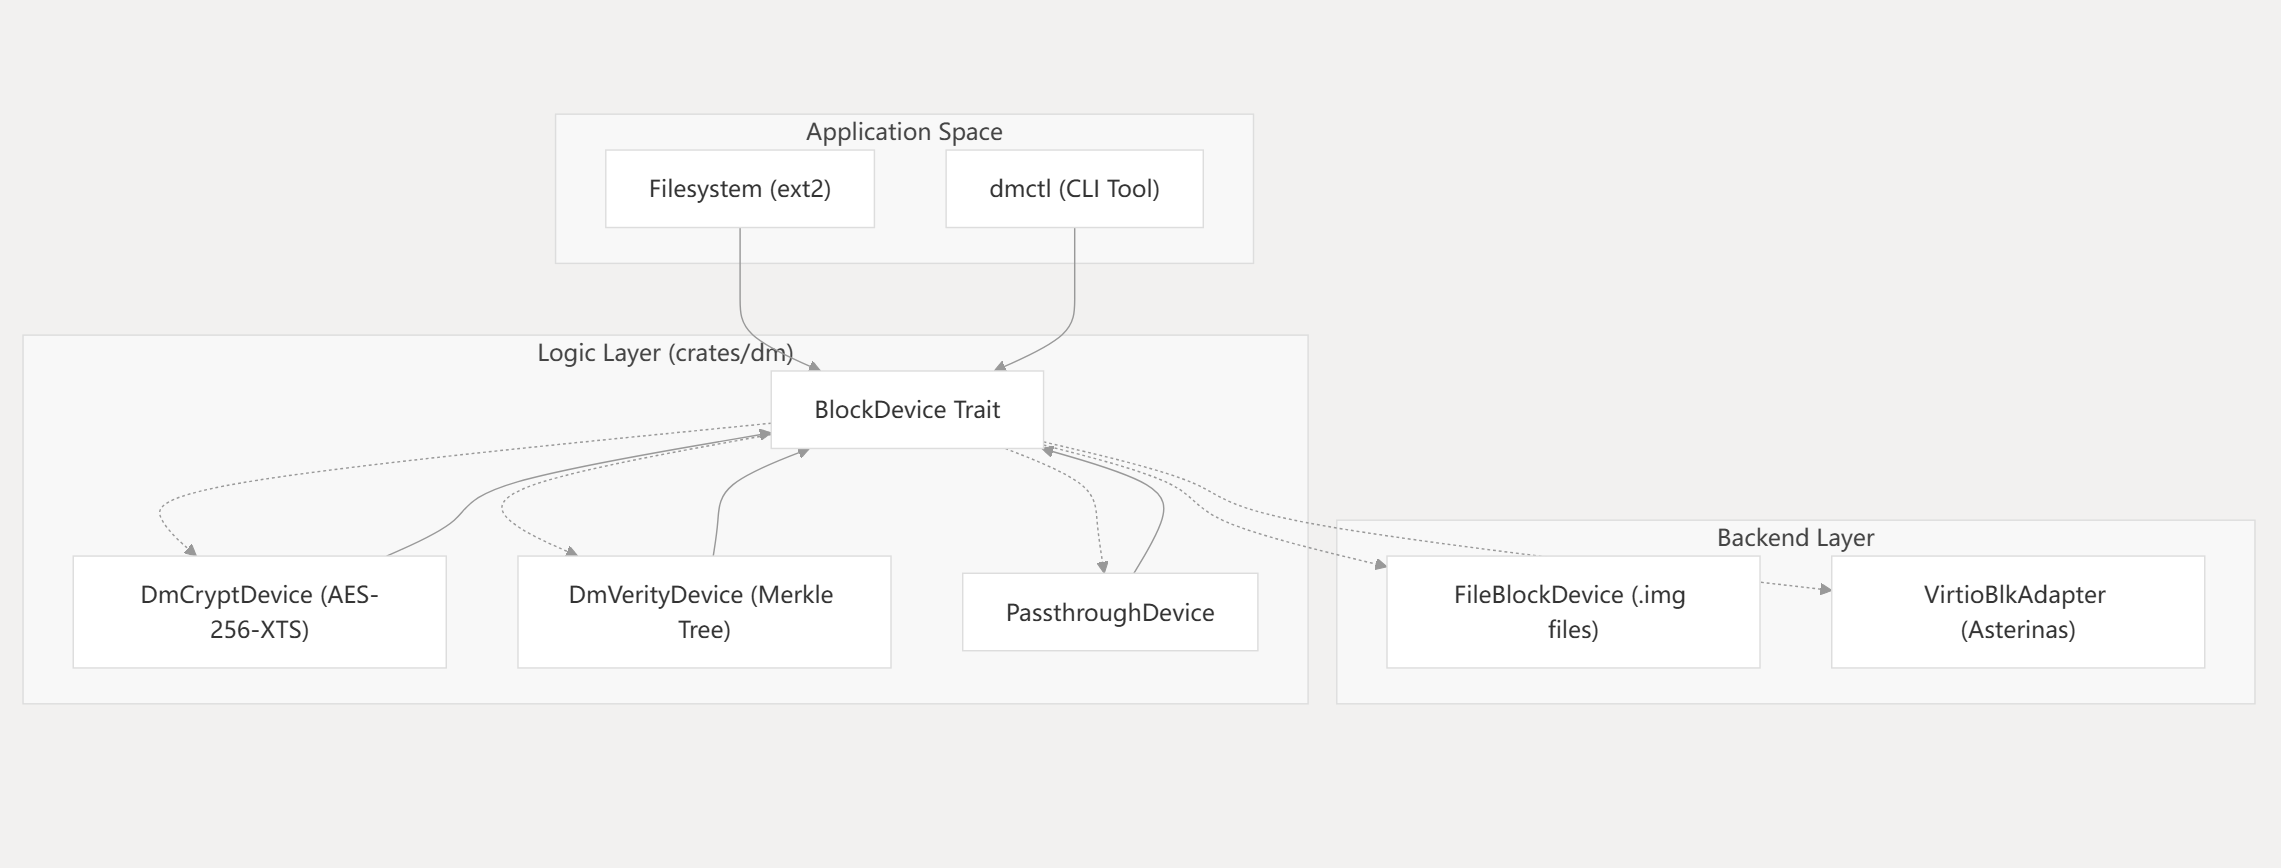
\includegraphics[width=0.85\textwidth]{figures/architecture.png}
    \caption{系统组件关系图}
    \label{fig:architecture}
\end{figure}

如图所示，文件系统或应用程序与顶层的 \texttt{BlockDevice}（例如 \texttt{DmCryptDevice}）交互，该设备在执行加密转换后，将 I/O 委托给下一层设备（如 \texttt{VirtioBlkAdapter} 或 \texttt{FileBlockDevice}），最终到达物理存储介质。

\section{文档结构}

本技术文档共分为九章和两个附录，结构如下：

\begin{itemize}
    \item \textbf{第2章 系统架构设计}：详细阐述 \texttt{BlockDevice} trait、可组合映射器链、模块分解及跨环境可移植性。
    \item \textbf{第3章 \texttt{dm-verity} 详细设计}：介绍默克尔树构建、单块校验路径、启动参数解析及只读强制策略。
    \item \textbf{第4章 \texttt{dm-crypt} 详细设计}：说明 \texttt{DmCryptTable}、AES-256-XTS 密码引擎、扇区算术及 Linux 兼容性验证。
    \item \textbf{第5章 性能优化策略}：涵盖哈希树缓存、零拷贝 I/O、批处理及硬件加速（AES-NI）等优化手段。
    \item \textbf{第6章 测试与性能分析报告}：包括功能正确性测试（篡改检测、明文/密文验证）、FIO 基准测试、启动开销分析及与 Linux 的交叉验证。
    \item \textbf{第7章 合规、来源与 AI 声明}：独立章节，严格遵循比赛要求，披露代码来源、开源协议及 AI 工具使用情况。
    \item \textbf{第8章 用户手册与部署指南}：提供从环境准备到编译、运行、配置的完整操作步骤。
    \item \textbf{第9章 研发过程与问题解决记录}：记录核心难题（如 Rust 所有权冲突、DMA 路径验证）及解决思路，并展示 Git 迭代历史。
    \item \textbf{附录 A 术语表}：定义代码库中的关键术语。
    \item \textbf{附录 B \texttt{dmctl} 命令参考}：列出所有子命令的签名、示例和实现说明。
\end{itemize}

\section{小结}

本章介绍了项目的背景、目标、双目标架构创新及整体文档结构。后续章节将深入阐述每个模块的设计与实现细节，并通过测试数据验证系统的功能正确性与性能表现。